\clearpage
\section{机电驱动模块建模}

%%%%%%%%%%%%%%%%%
\begin{figure*}[!h]
	\centering
	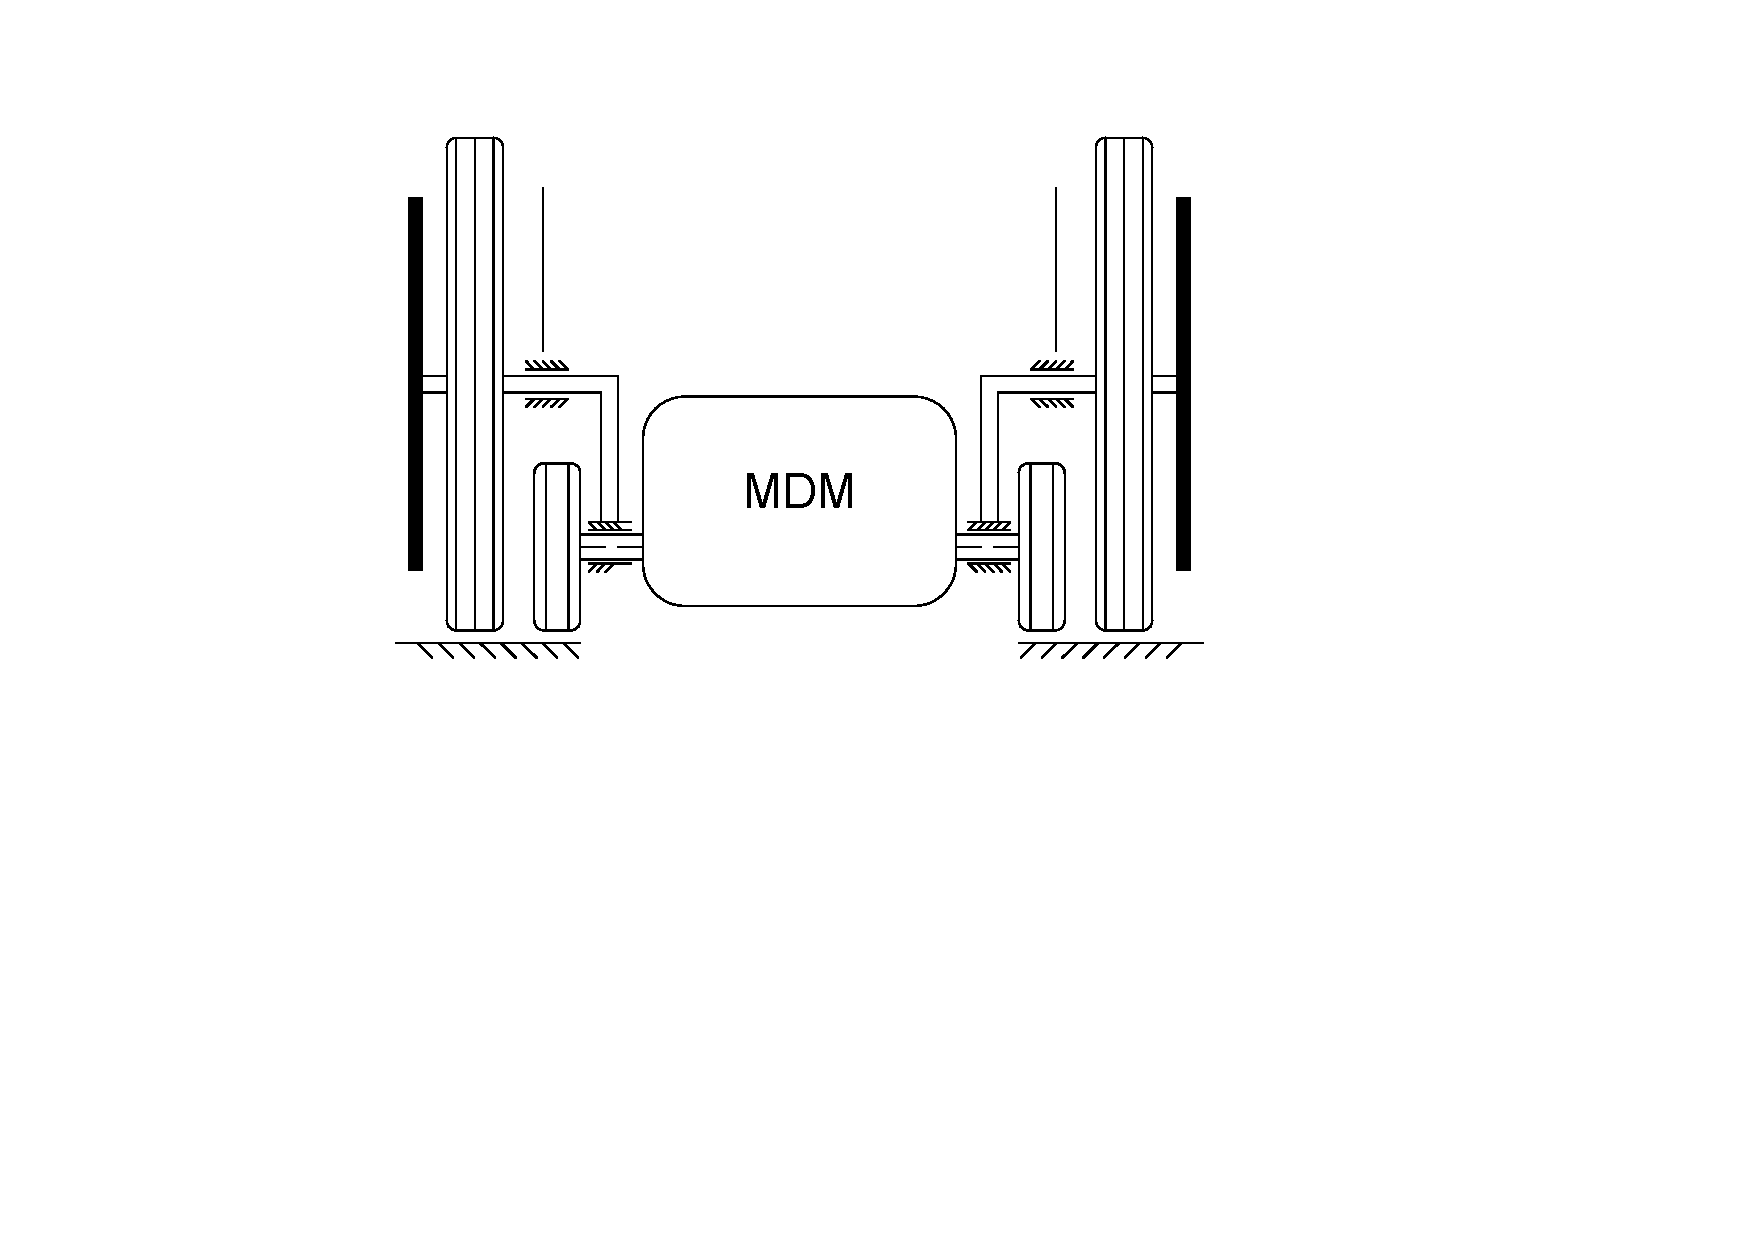
\includegraphics[width=0.6\textwidth]{fig/MDM_modified.pdf}
	\caption{机电驱动模块(MDM, \textit{mechatronic drive module})简图。}\label{fig:MDM_modified} % schematic diagram
\end{figure*}
%%%%%%%%%%%%%%%%%

为了研究有助于系统动态行为的不同组件,机电驱动模块与主体结构分离,基本布局如图~\ref{fig:MDM_modified} 所示。它包括使用速度减小的机械齿轮以及电动轮连接到系统的方式。轴上的旋转阻尼器和扭转弹簧的小值已经集中在一起并分别由 $R_s$ 和 $C_s$ 表示。

由此我们构建了相关的键图模型,它仅代表从电动推进轮椅中提取的机电一体化驱动模块系统如图~\ref{fig:MDM_scheme} 所示的动态特性的组件。

%%%%%%%%%%%%%%%%%
\begin{figure*}[!h]
	\centering
	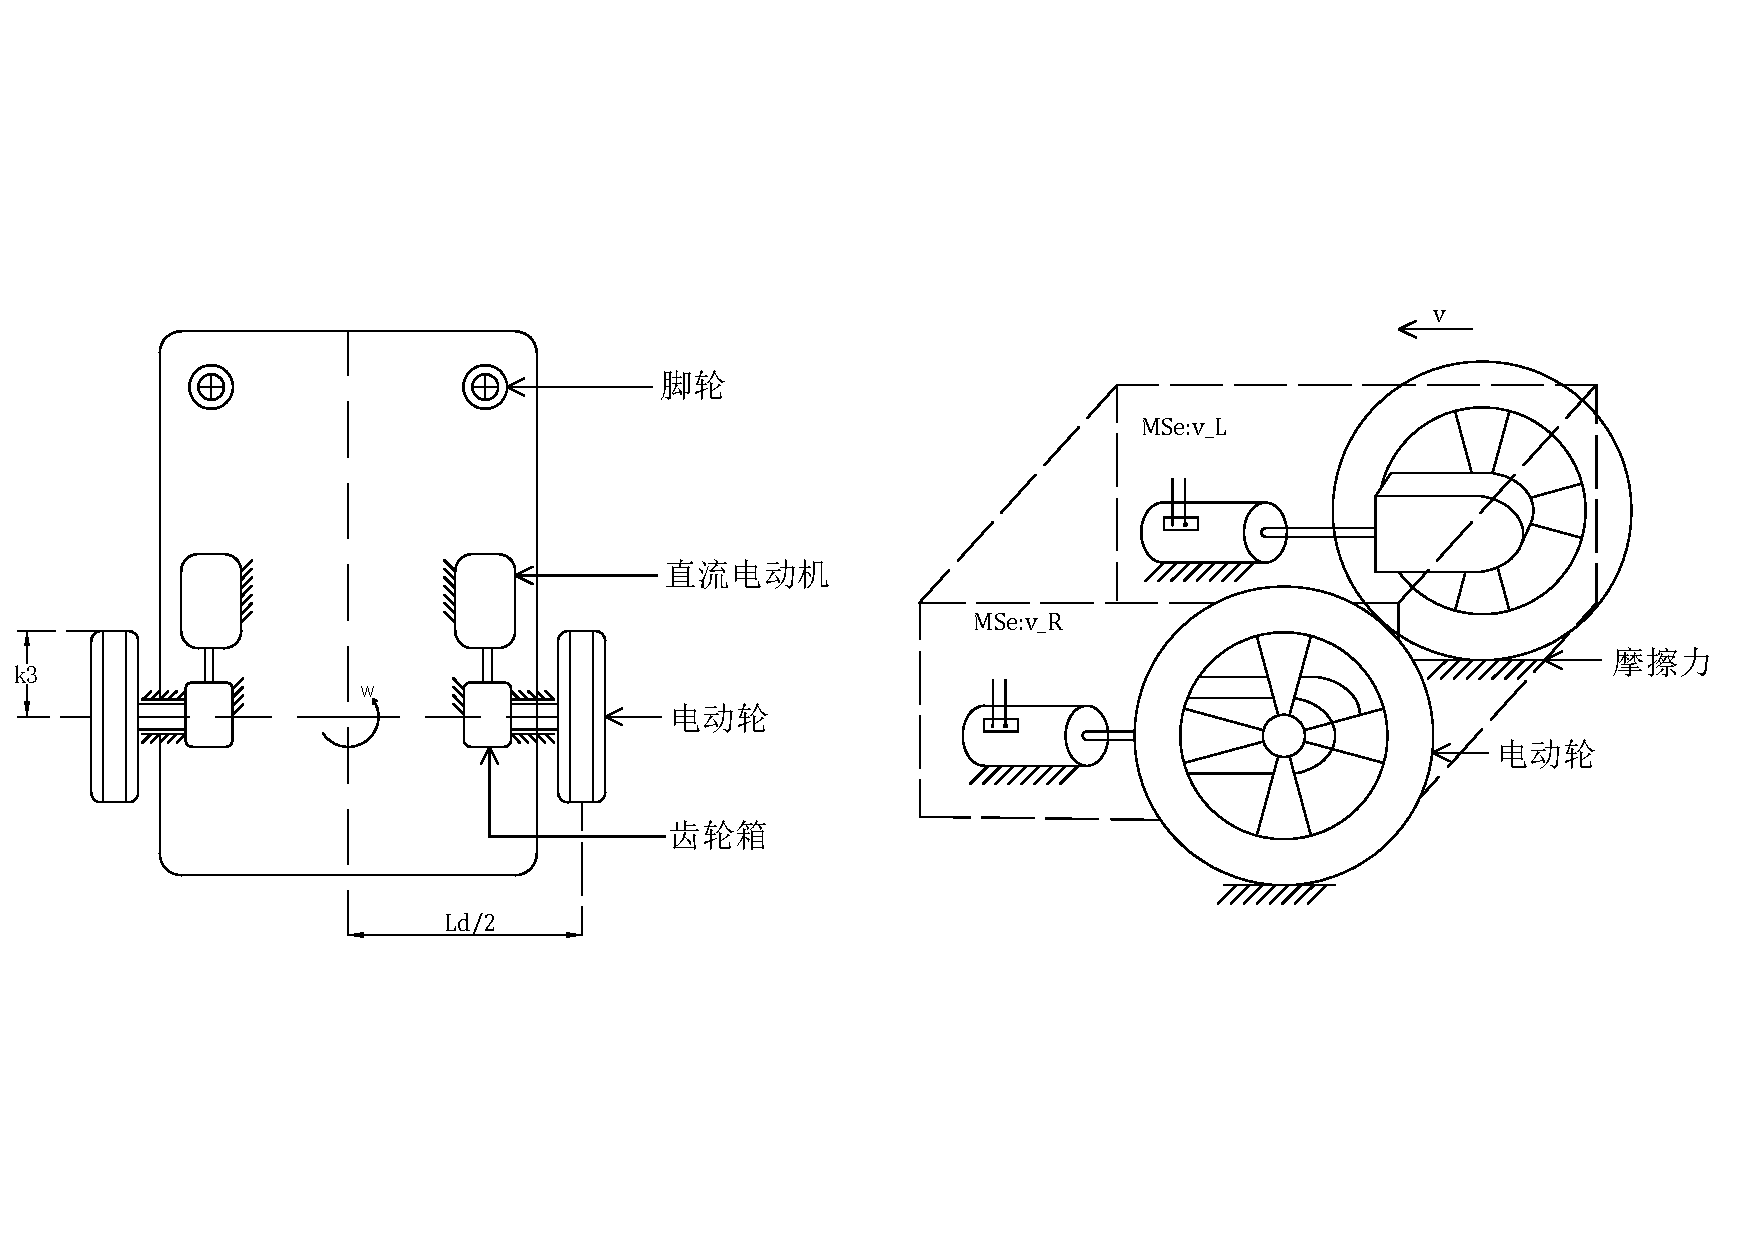
\includegraphics[width=1\textwidth]{fig/MDM_scheme.pdf}
	\caption{机电驱动模块主要结构示意。}\label{fig:MDM_scheme} % schematic diagram
\end{figure*}
%%%%%%%%%%%%%%%%%

\clearpage

\subsection{电机模块键合图及其导出过程}

首先对他励直流电机进行分析建模。作为机电驱动模块的核心,该部分我们既考虑了电路结构(包括主电路以及他励电路),也考虑了在输出扭矩时的机械损失。

我们用 MSe:L,$ I_e $,$ R_e $ 来分别表示输入控制电压,电机电感和内阻;用 $ J_r $,$ R_b $,$ C_s $,$ R_s $,$ k_1 $来分别表示转子转动惯量,电机轴承阻尼,电机输出转矩,电机输出轴阻尼和电机扭矩系数。如下图~\ref{fig:separately_excited_dc_motor}可见。根据电系统特点,我们标出相关共势点,为后续分析做准备。

%%%%%%%%%%%%%%%%%
\begin{figure*}[!h]
	\centering
	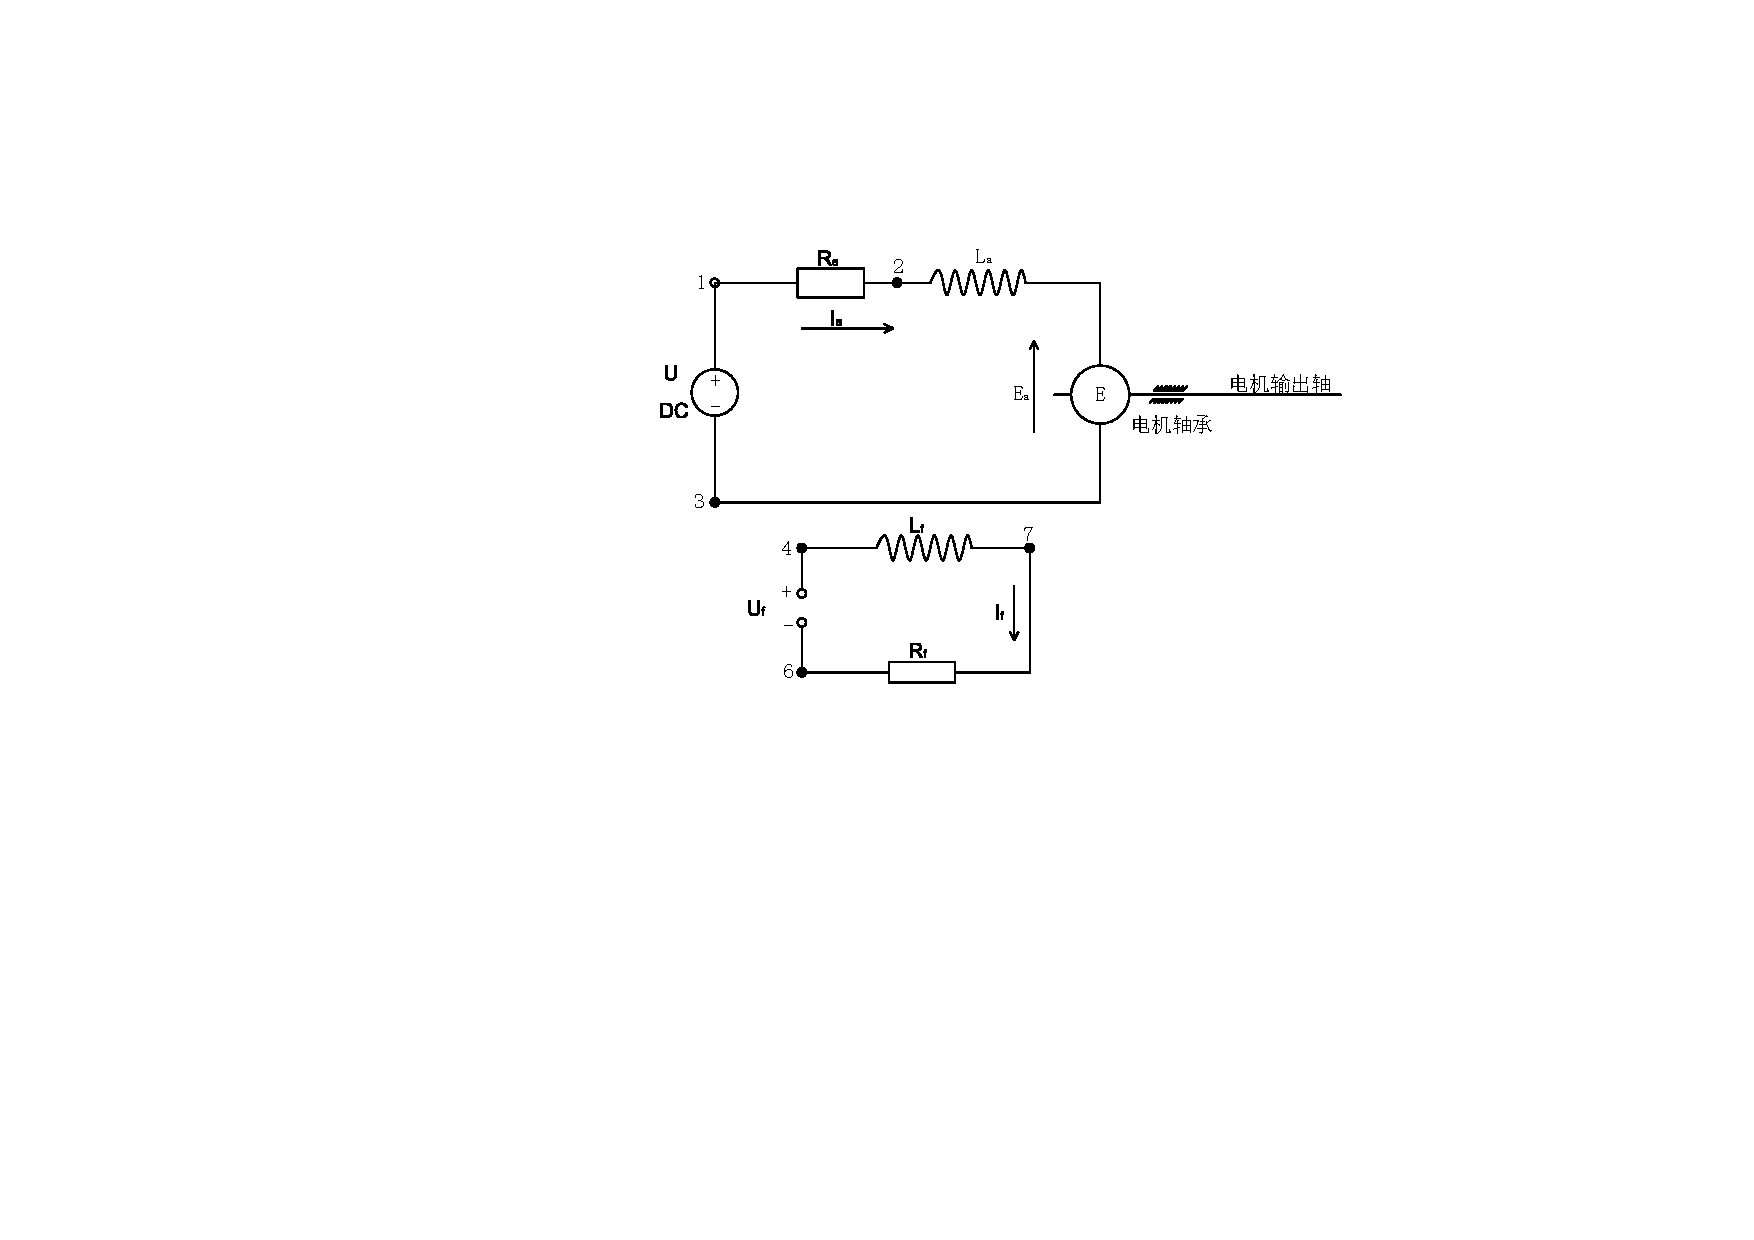
\includegraphics[width=1.05\textwidth]{fig/separately_excited_dc_motor.pdf}
	\caption{他励直流电机原理简图。}\label{fig:separately_excited_dc_motor} % schematic diagram
\end{figure*}
%%%%%%%%%%%%%%%%%

以下为具体建模过程:

\begin{enumerate}
	\item 定义电流的正方向以及电机输出轴的转速正方向如图~\ref{fig:separately_excited_dc_motor} 所示。
	
	\item 电路主回路和励磁回路分别有3个共势点,电机轴包括2个速度结点。
	如下图所示:
	%%%%%%%%%%%%%%%%%
	\begin{figure*}[!h]
		\centering
		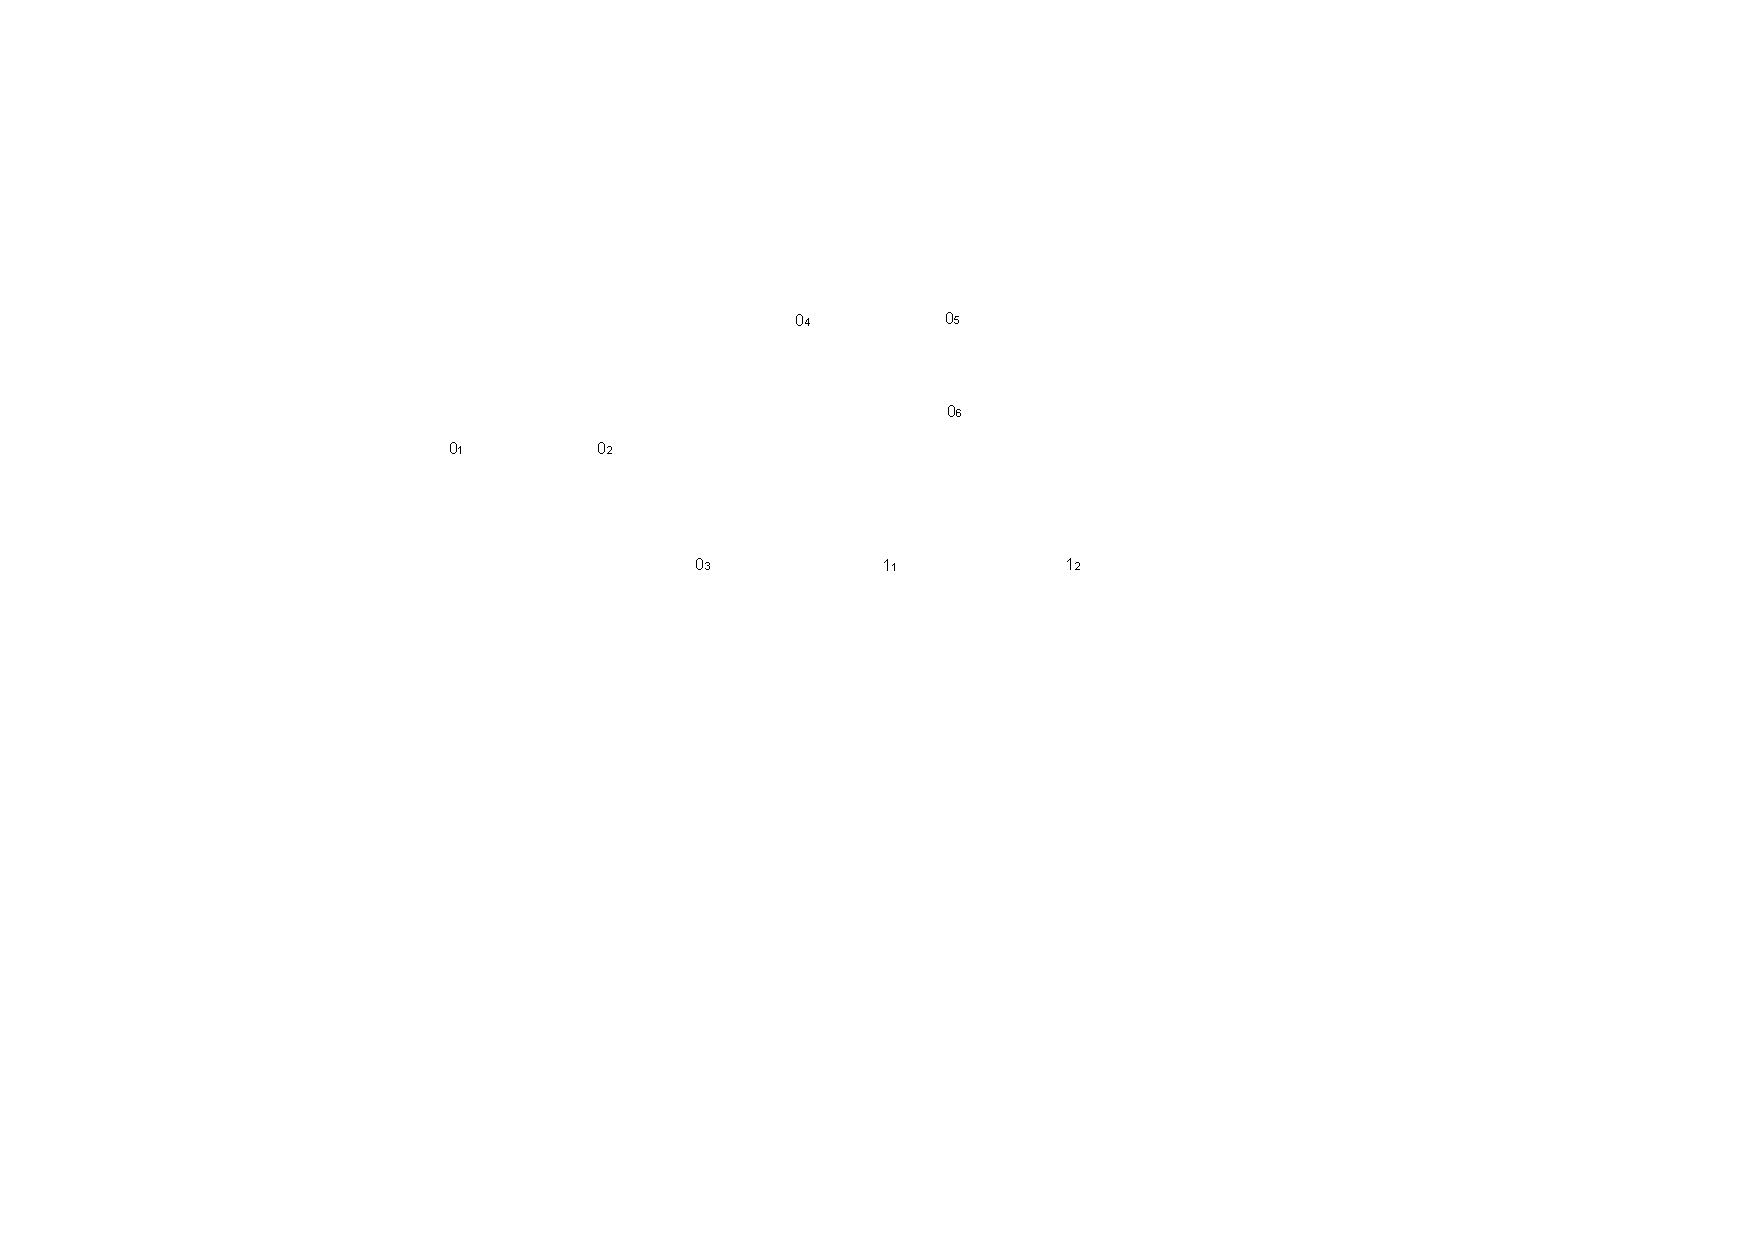
\includegraphics[width=1.05\textwidth]{fig/4_1_bond.pdf}
		\caption{标注0-结与1-结。}\label{fig:4_1_bond}
	\end{figure*}
	%%%%%%%%%%%%%%%%%
	
	\clearpage
	
	\item 添加源和RCI元件。同时根据功率方向画出半箭头。
	如下图所示:
	%%%%%%%%%%%%%%%%%
	\begin{figure*}[!h]
		\centering
		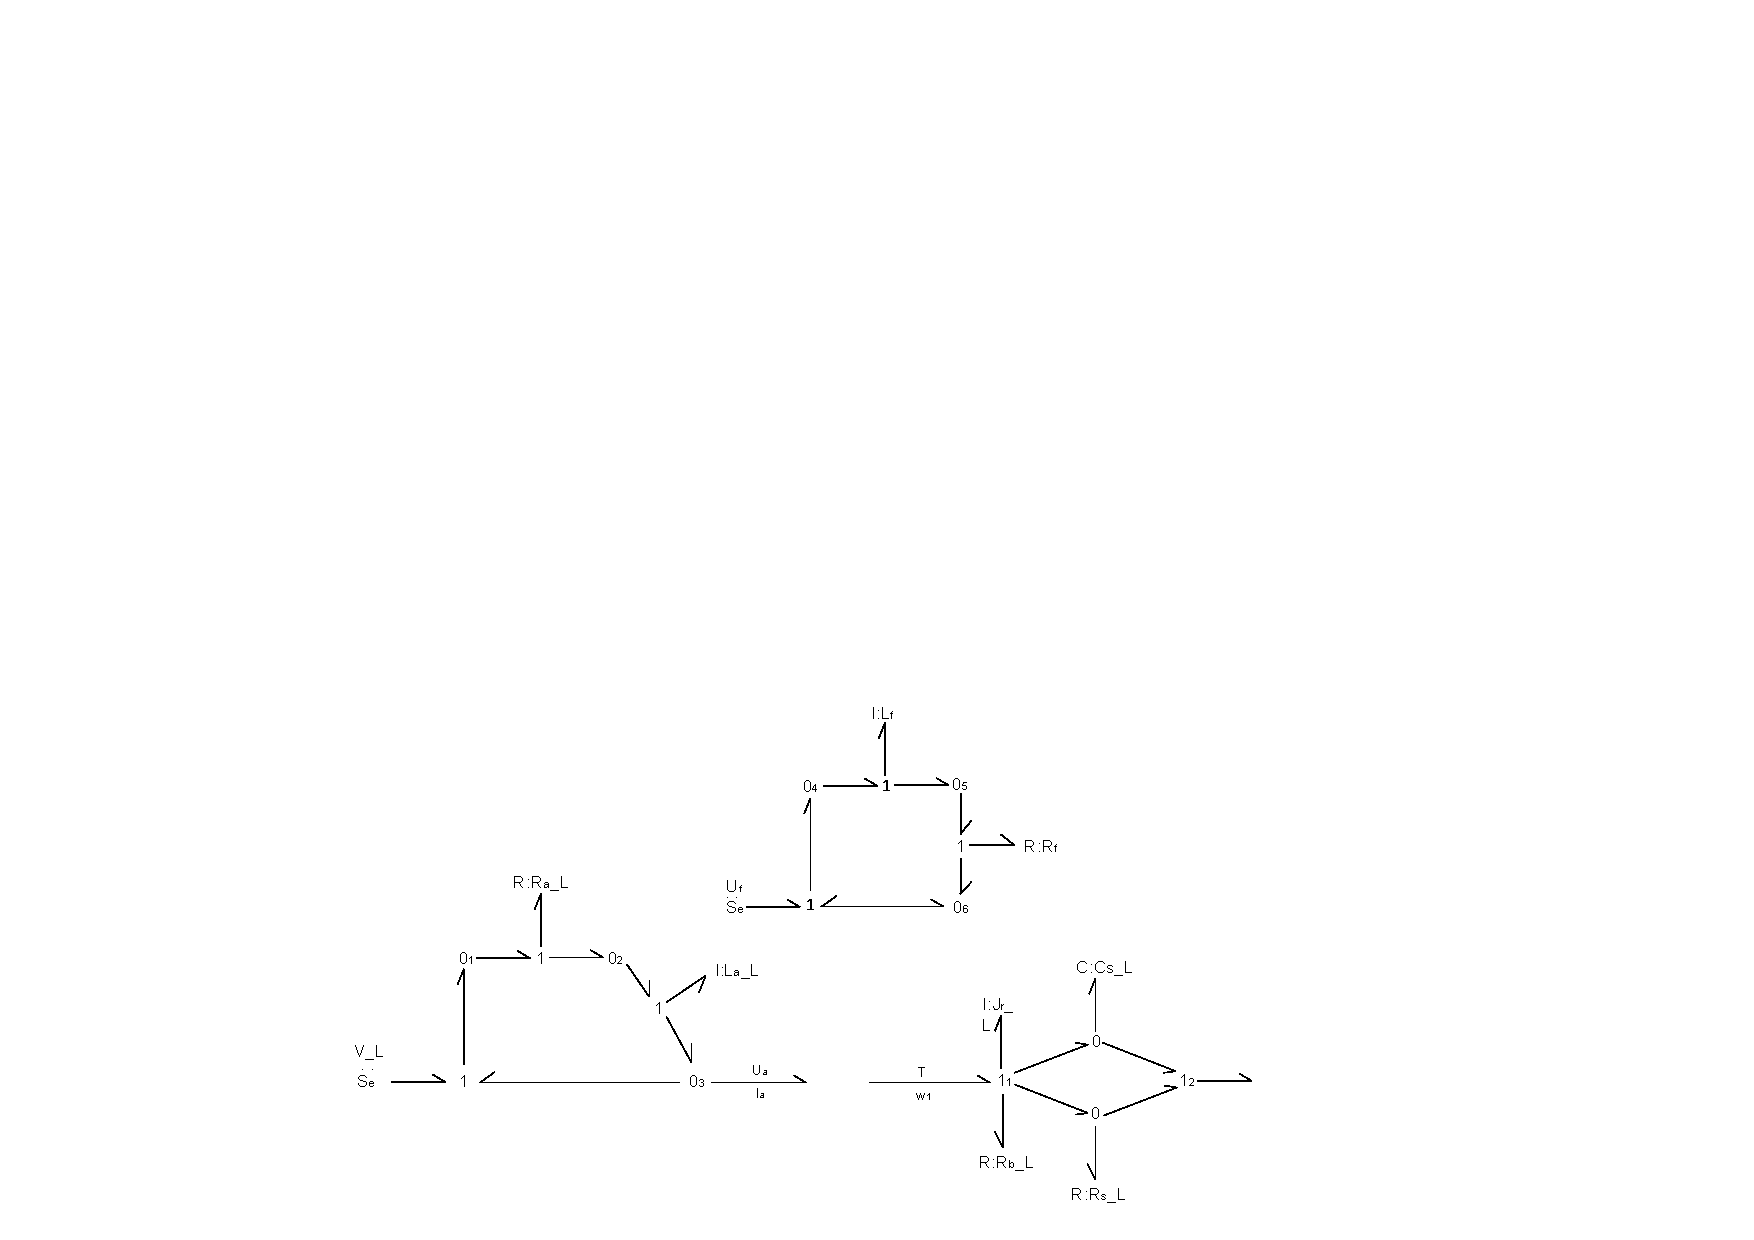
\includegraphics[width=0.92\textwidth]{fig/4_2_bond.pdf}
		\caption{添加源和RCI元件。}\label{fig:4_2_bond}
	\end{figure*}
	%%%%%%%%%%%%%%%%%
	
	\item 在电系统和机械系统之间添加回转器。根据对应数学关系:
	%%%%%%%%%%%%%%%%%%%%%%%%%%
	\begin{equation}
	\label{equ:U_a}
	U_a
	=
	\left( C_e \Phi_e \frac{60}{2 \pi}\right) * w_1
	\ ,
	\end{equation}
	%%%%%%%%%%%%%%%%%%%%%%%%%%
	%%%%%%%%%%%%%%%%%%%%%%%%%%
	\begin{equation}
	\label{equ:U_a}
	T
	=\
	(C_t \Phi_e) * I_a
	\ .
	\end{equation}
	%%%%%%%%%%%%%%%%%%%%%%%%%%
	
	同时根据功率方向画出半箭头。
	如下图所示:	
	%%%%%%%%%%%%%%%%%
	\begin{figure*}[!h]
		\centering
		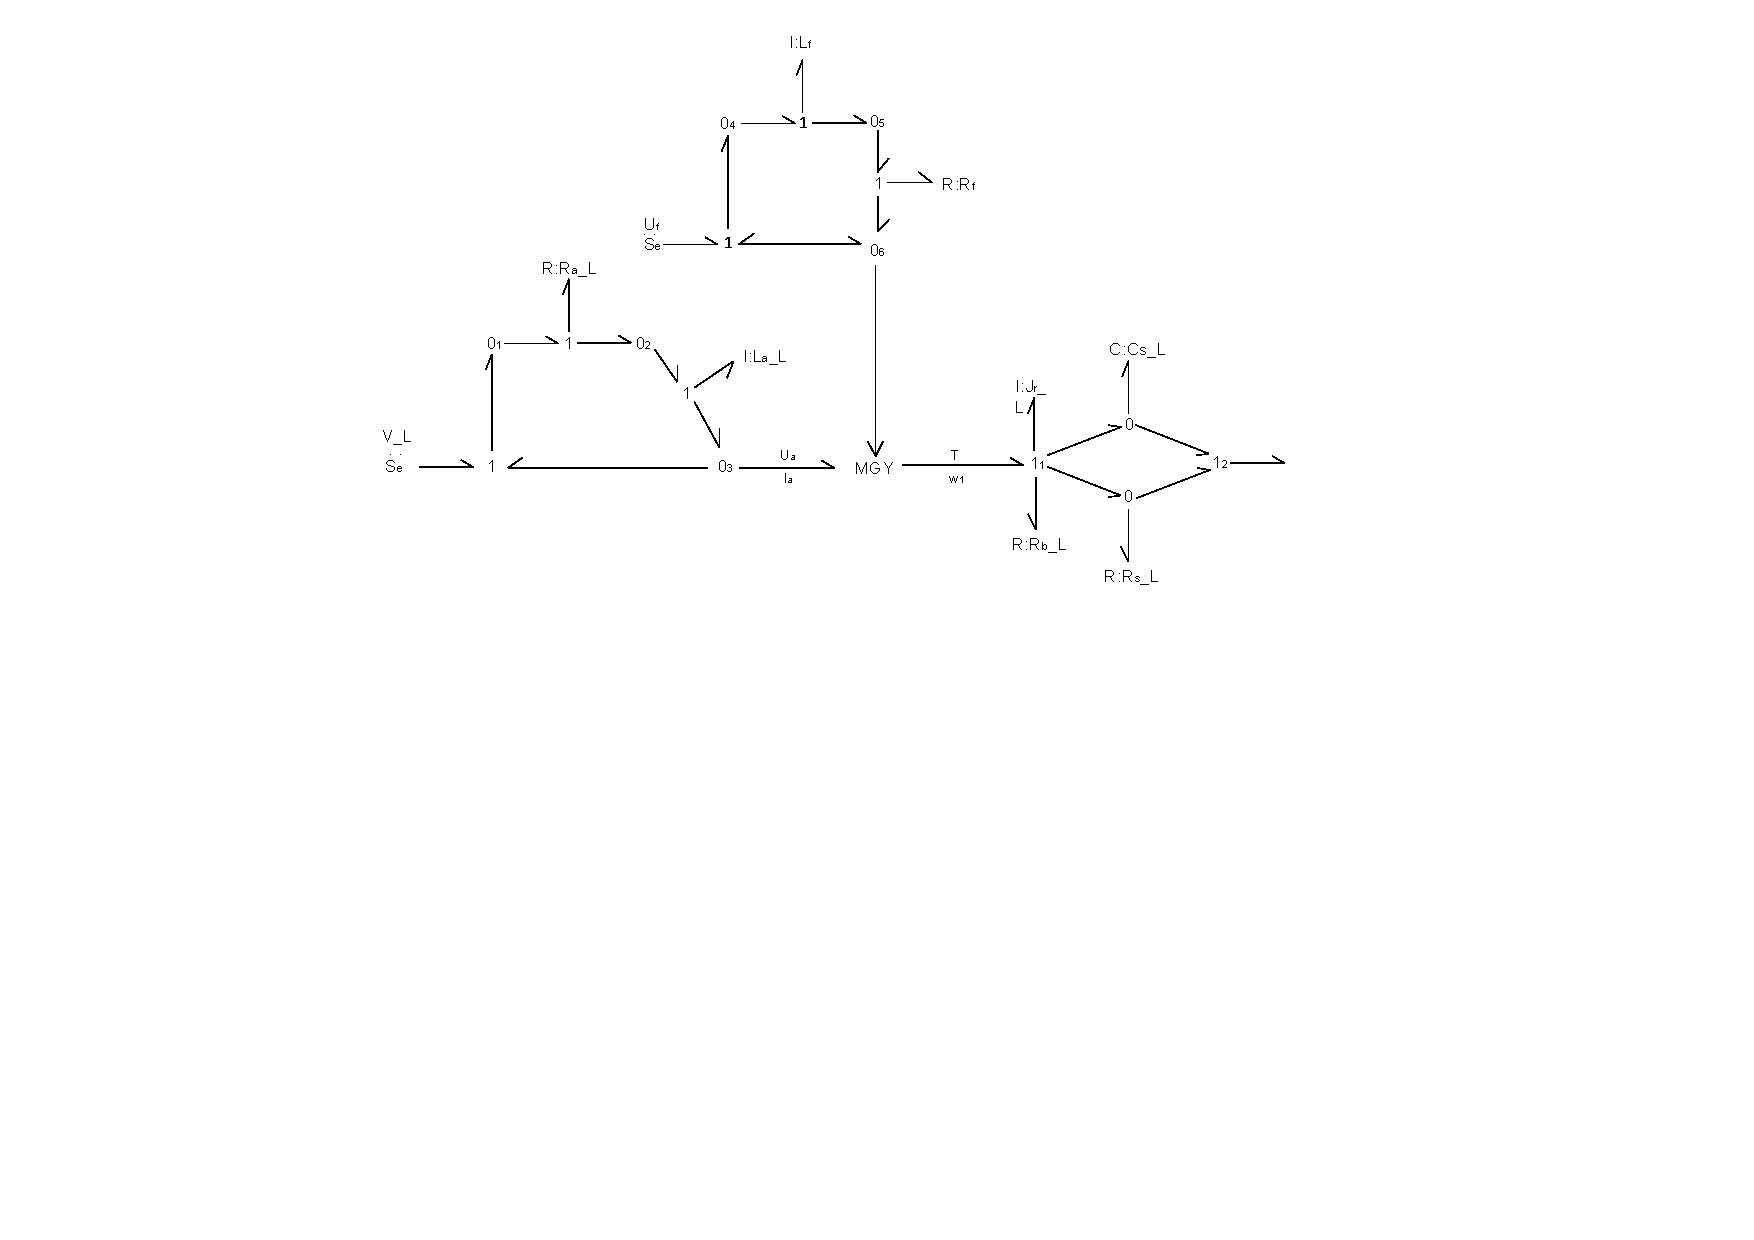
\includegraphics[width=0.92\textwidth]{fig/4_3_bond.pdf}
		\caption{添加回转器。}\label{fig:4_3_bond}
	\end{figure*}
	%%%%%%%%%%%%%%%%%
	
	\item 电机模型电系统部分化简。根据电路图可知,03和06接地,因此可以对上面键合图进行化简。
	如下图所示:
	%%%%%%%%%%%%%%%%%
	\begin{figure*}[!h]
		\centering
		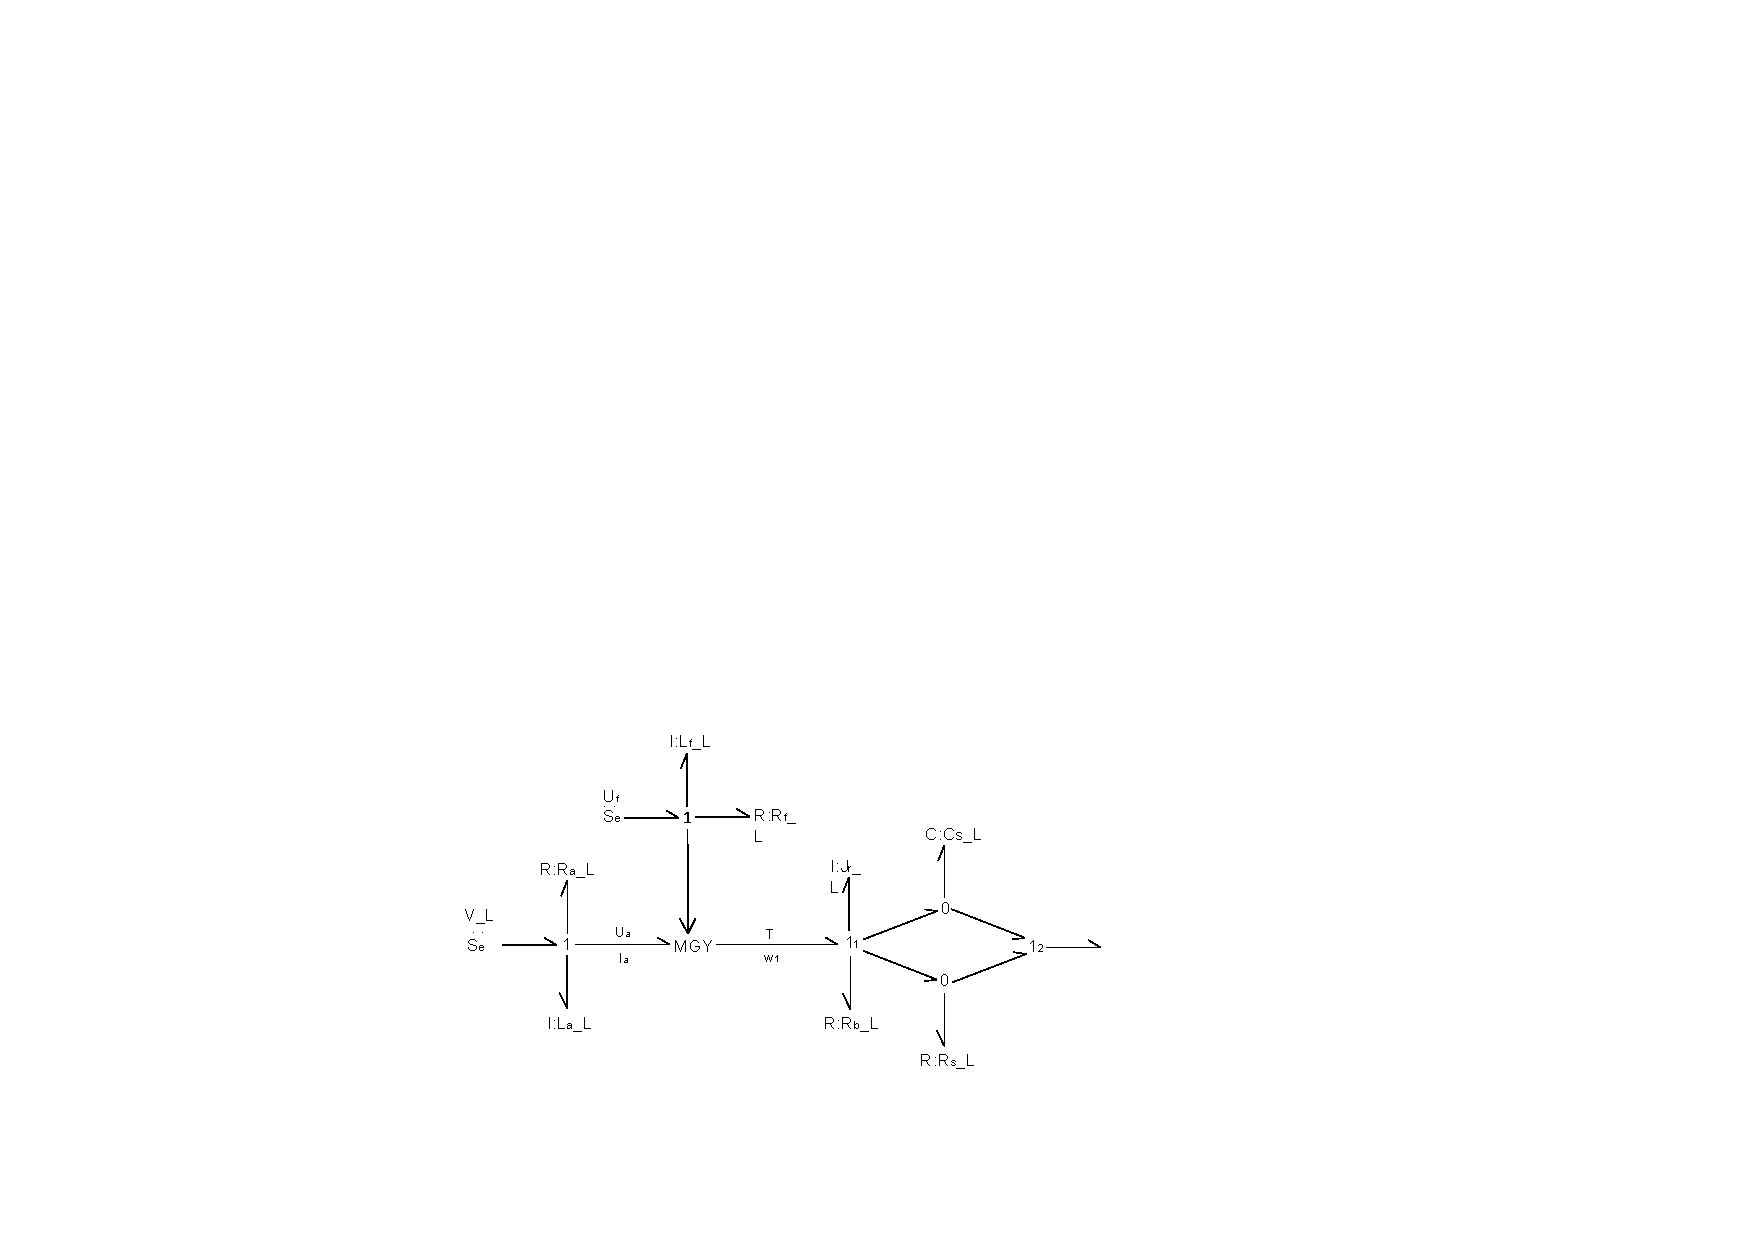
\includegraphics[width=1.2\textwidth]{fig/4_4_bond.pdf}
		\caption{电机模型电系统部分化简。}\label{fig:4_4_bond}
	\end{figure*}
	%%%%%%%%%%%%%%%%%
	
	\item 电机模型功率环化简。
	如下图所示:
	%%%%%%%%%%%%%%%%%
	\begin{figure*}[!h]
		\centering
		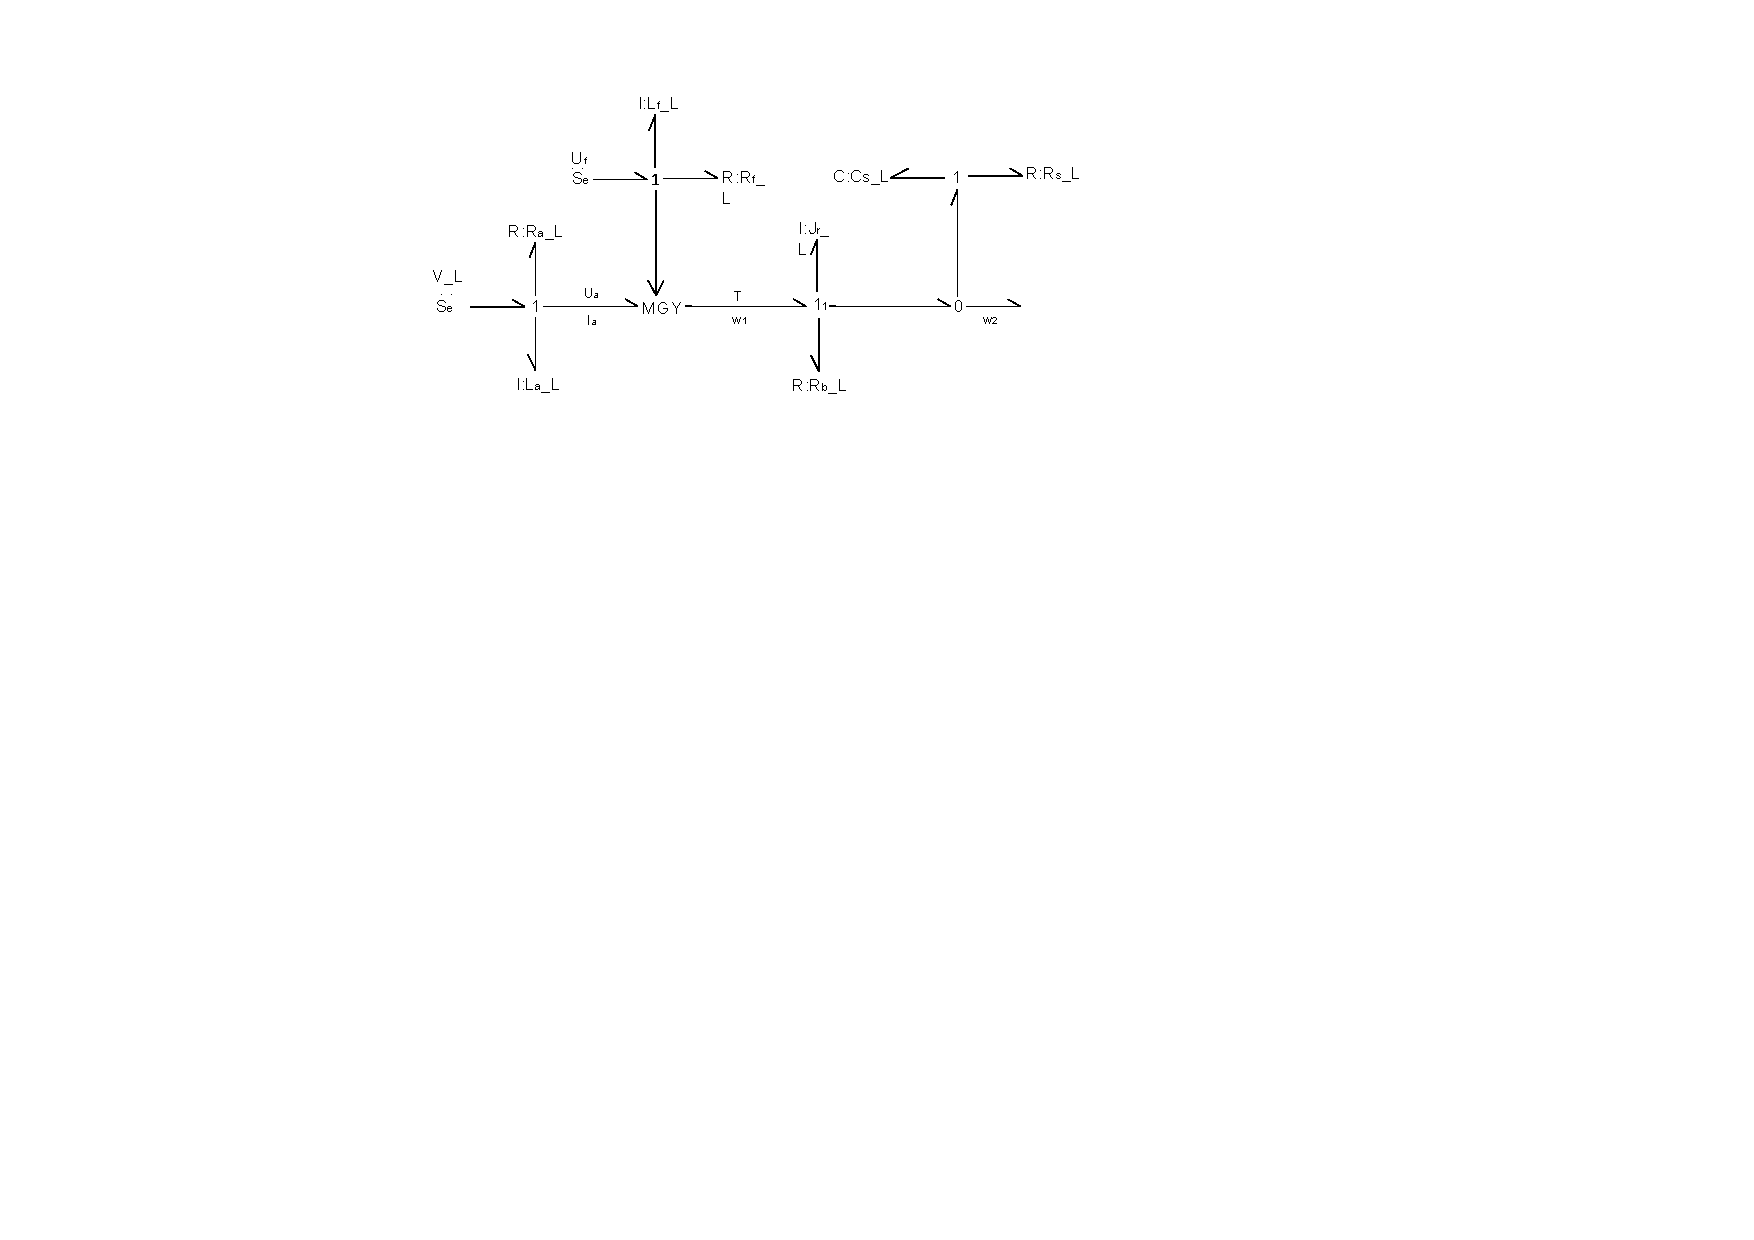
\includegraphics[width=1\textwidth]{fig/4_5_bond.pdf}
		\caption{电机模型功率环化简。}\label{fig:4_5_bond}
	\end{figure*}
	%%%%%%%%%%%%%%%%%
	
\end{enumerate}

\clearpage

\subsection{电驱动模块其余部分键合图}

以下为具体建模过程:

\begin{enumerate}
	\item 对于每一个确定的速度,标注速度1-结。
	本装置一共有 6 个确定的(角)速度,即左/右后轮角速度,左/右后轮线速度,电驱动模块质心速度和电驱动模块质心角速度。
	如下图所示:
	%%%%%%%%%%%%%%%%%
	\begin{figure*}[!h]
		\centering
		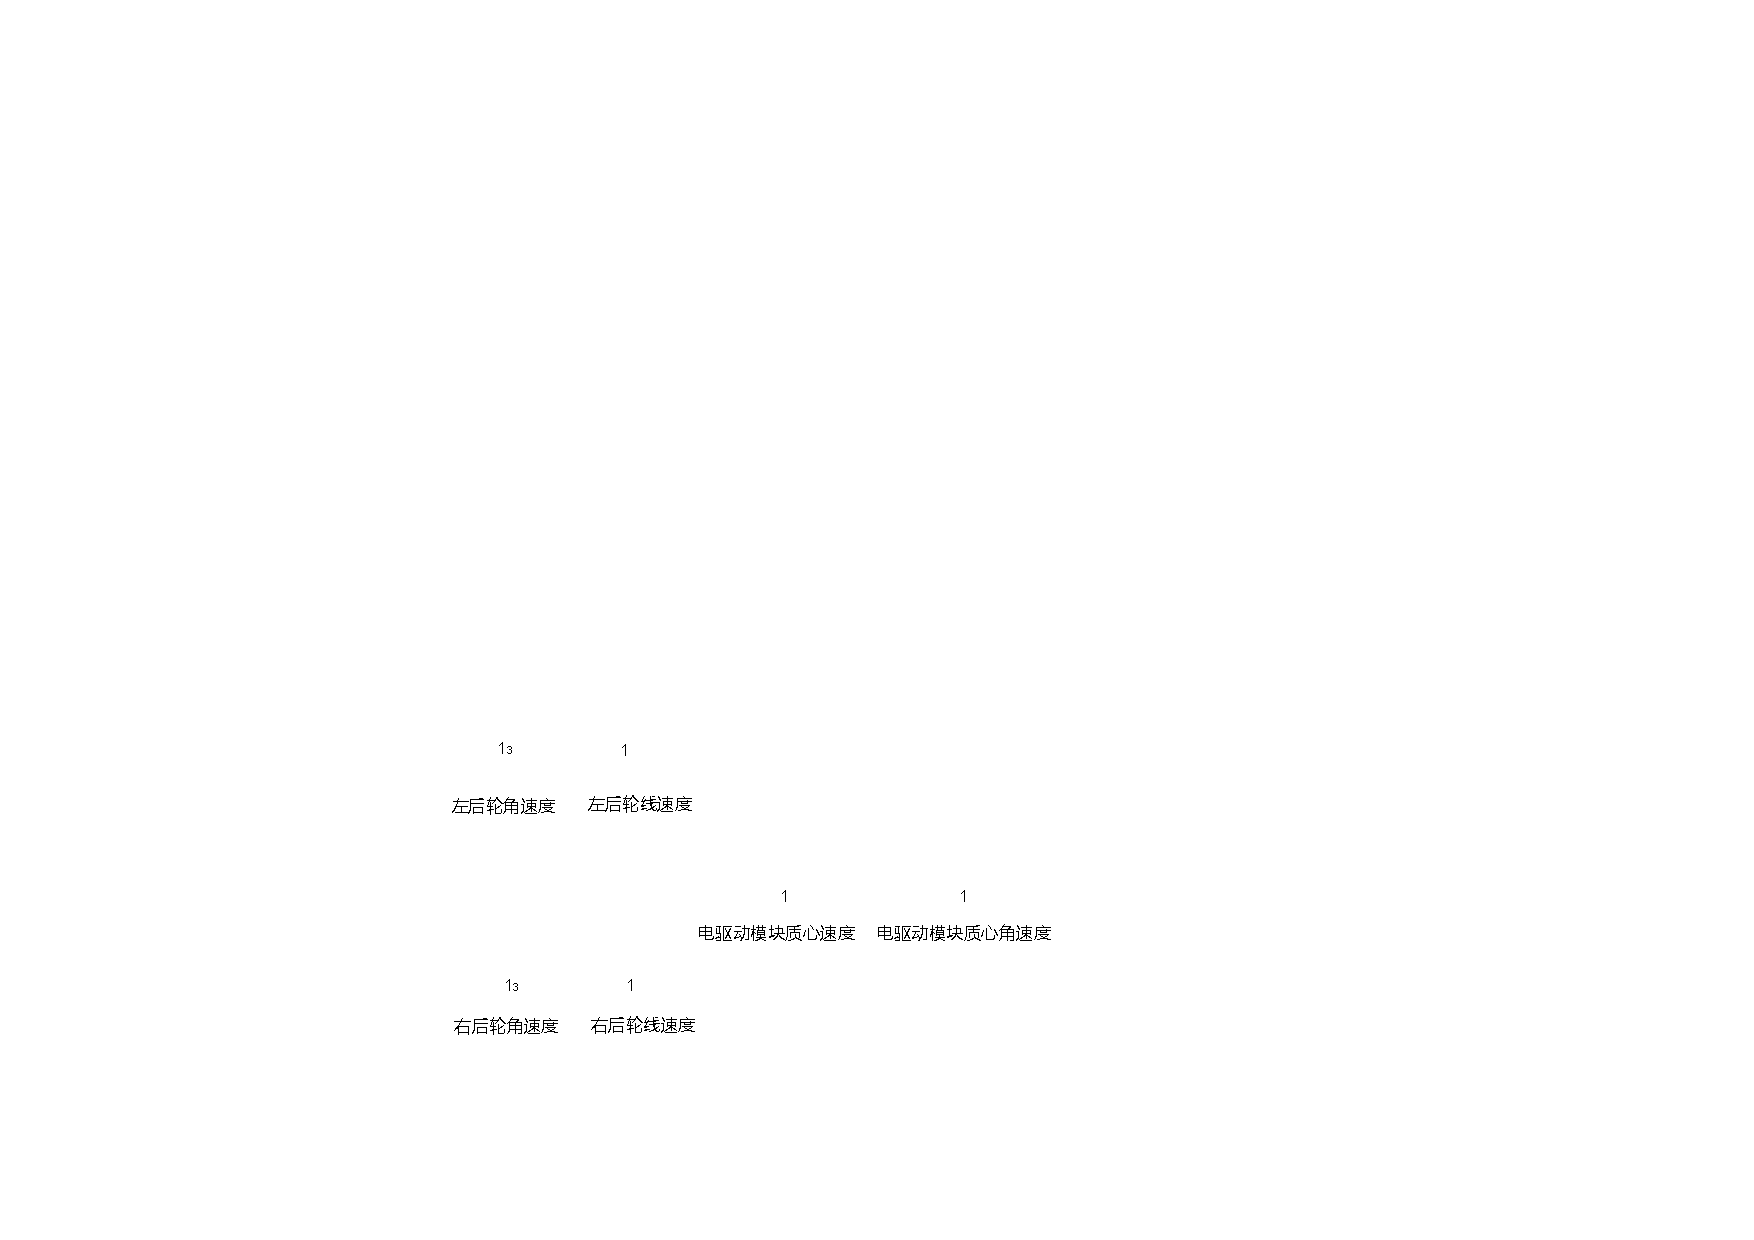
\includegraphics[width=0.75\textwidth]{fig/4_6_bond.pdf}
		\caption{标注速度1-结。}\label{fig:4_6_bond}
	\end{figure*}
	%%%%%%%%%%%%%%%%%
	
	\item 添加RCI元件。同时根据功率方向画出半箭头。
	如下图所示:
	%%%%%%%%%%%%%%%%%
	\begin{figure*}[!h]
		\centering
		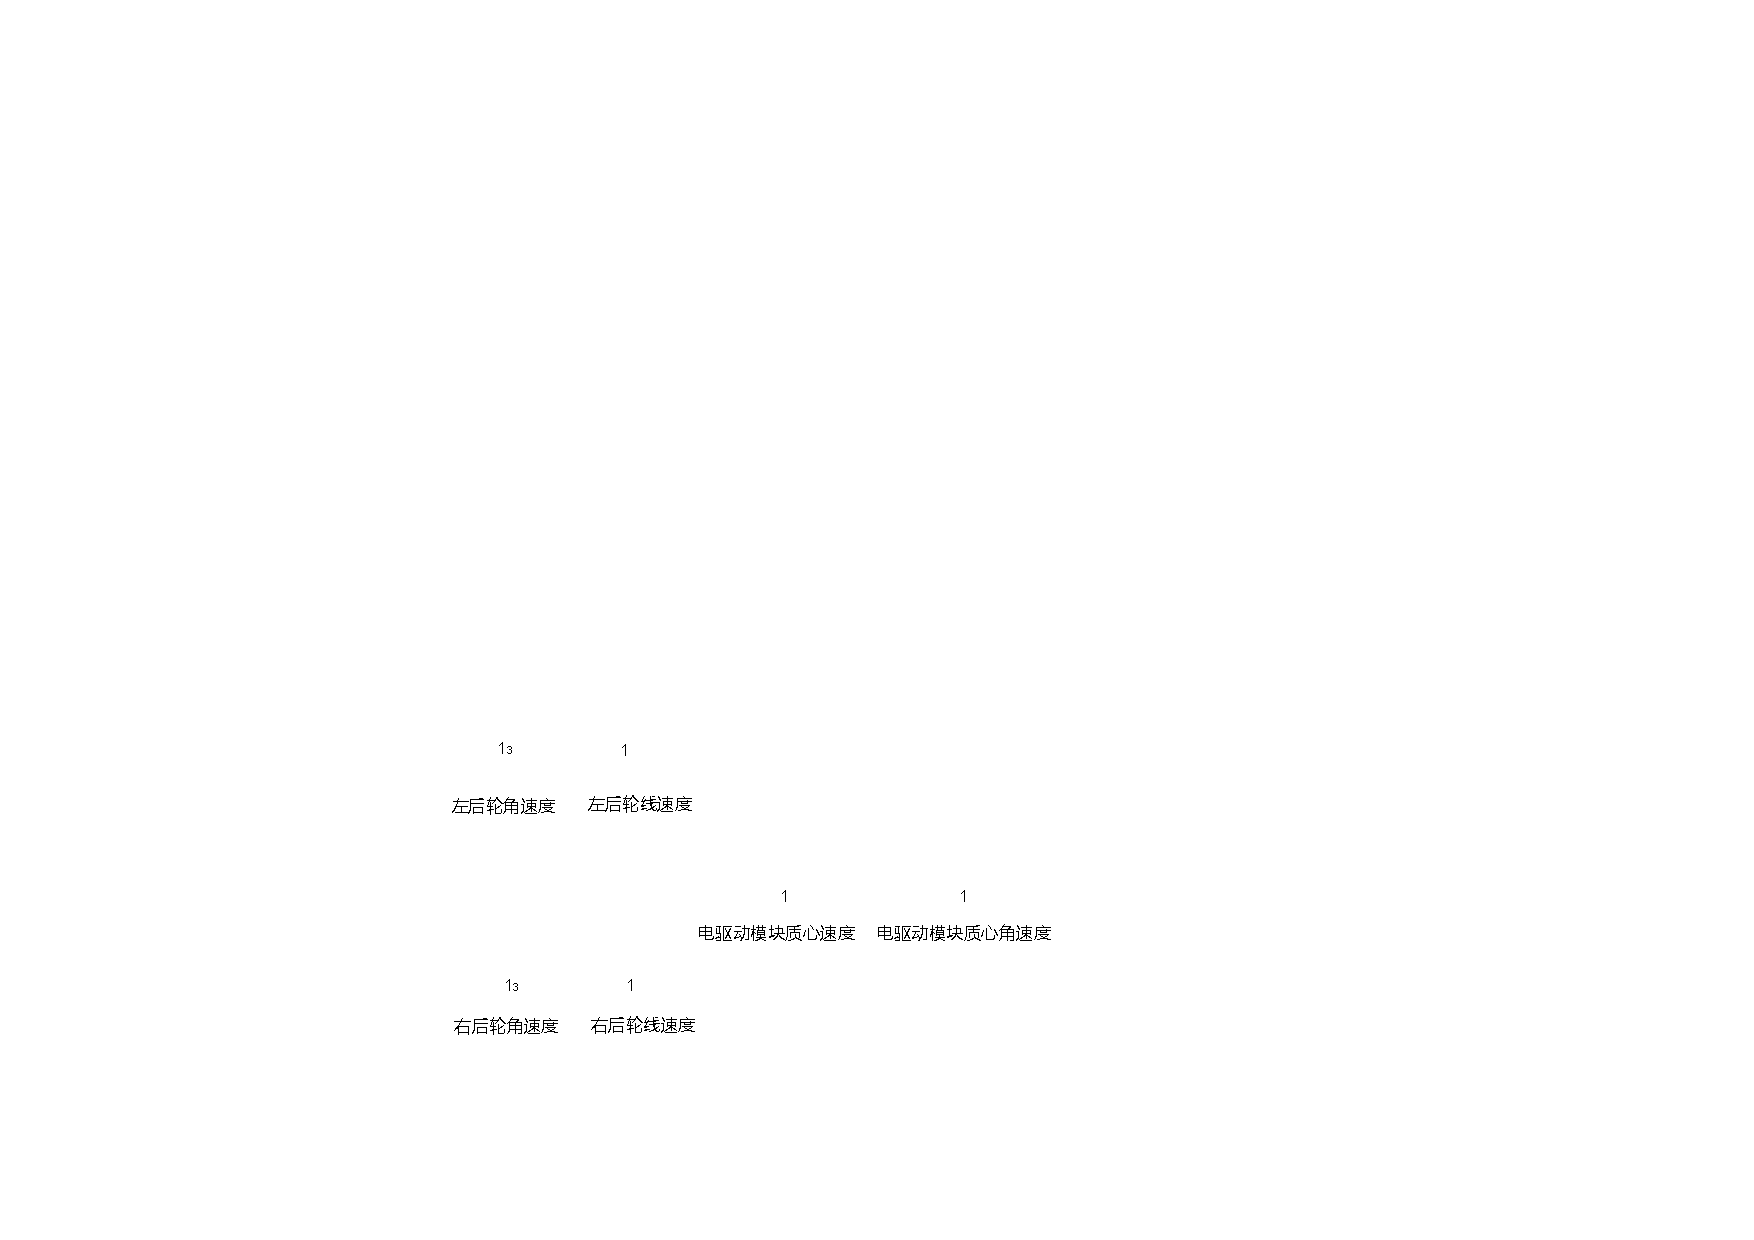
\includegraphics[width=0.8\textwidth]{fig/4_6_bond.pdf}
		\caption{电机模型电系统部分化简。}\label{fig:4_7_bond}
	\end{figure*}
	%%%%%%%%%%%%%%%%%
	
	
\end{enumerate}

\clearpage

\subsection{机电驱动模块键合图}

相比于图xxx和图xxx,他励直流电动机与电动小车机械部分结合,它们之间通过一个减速齿轮箱连接,所以键合图连接的地方需要添加一个变换器。

最终得到构成机电驱动模块的各个部件组件的键合图,如图~\ref{fig:part2_bond} 示,该键合图模型分解为四个主要部分,前两个代表电动机和传动齿轮,而第二个显示车轮惯性,最后一个显示围绕整车质量 $M_d$ 和转动惯量 $J_d$ 惯性建立的轮椅结构的动力学。

%%%%%%%%%%%%%%%%%
\begin{figure*}[!h]
	\centering
	%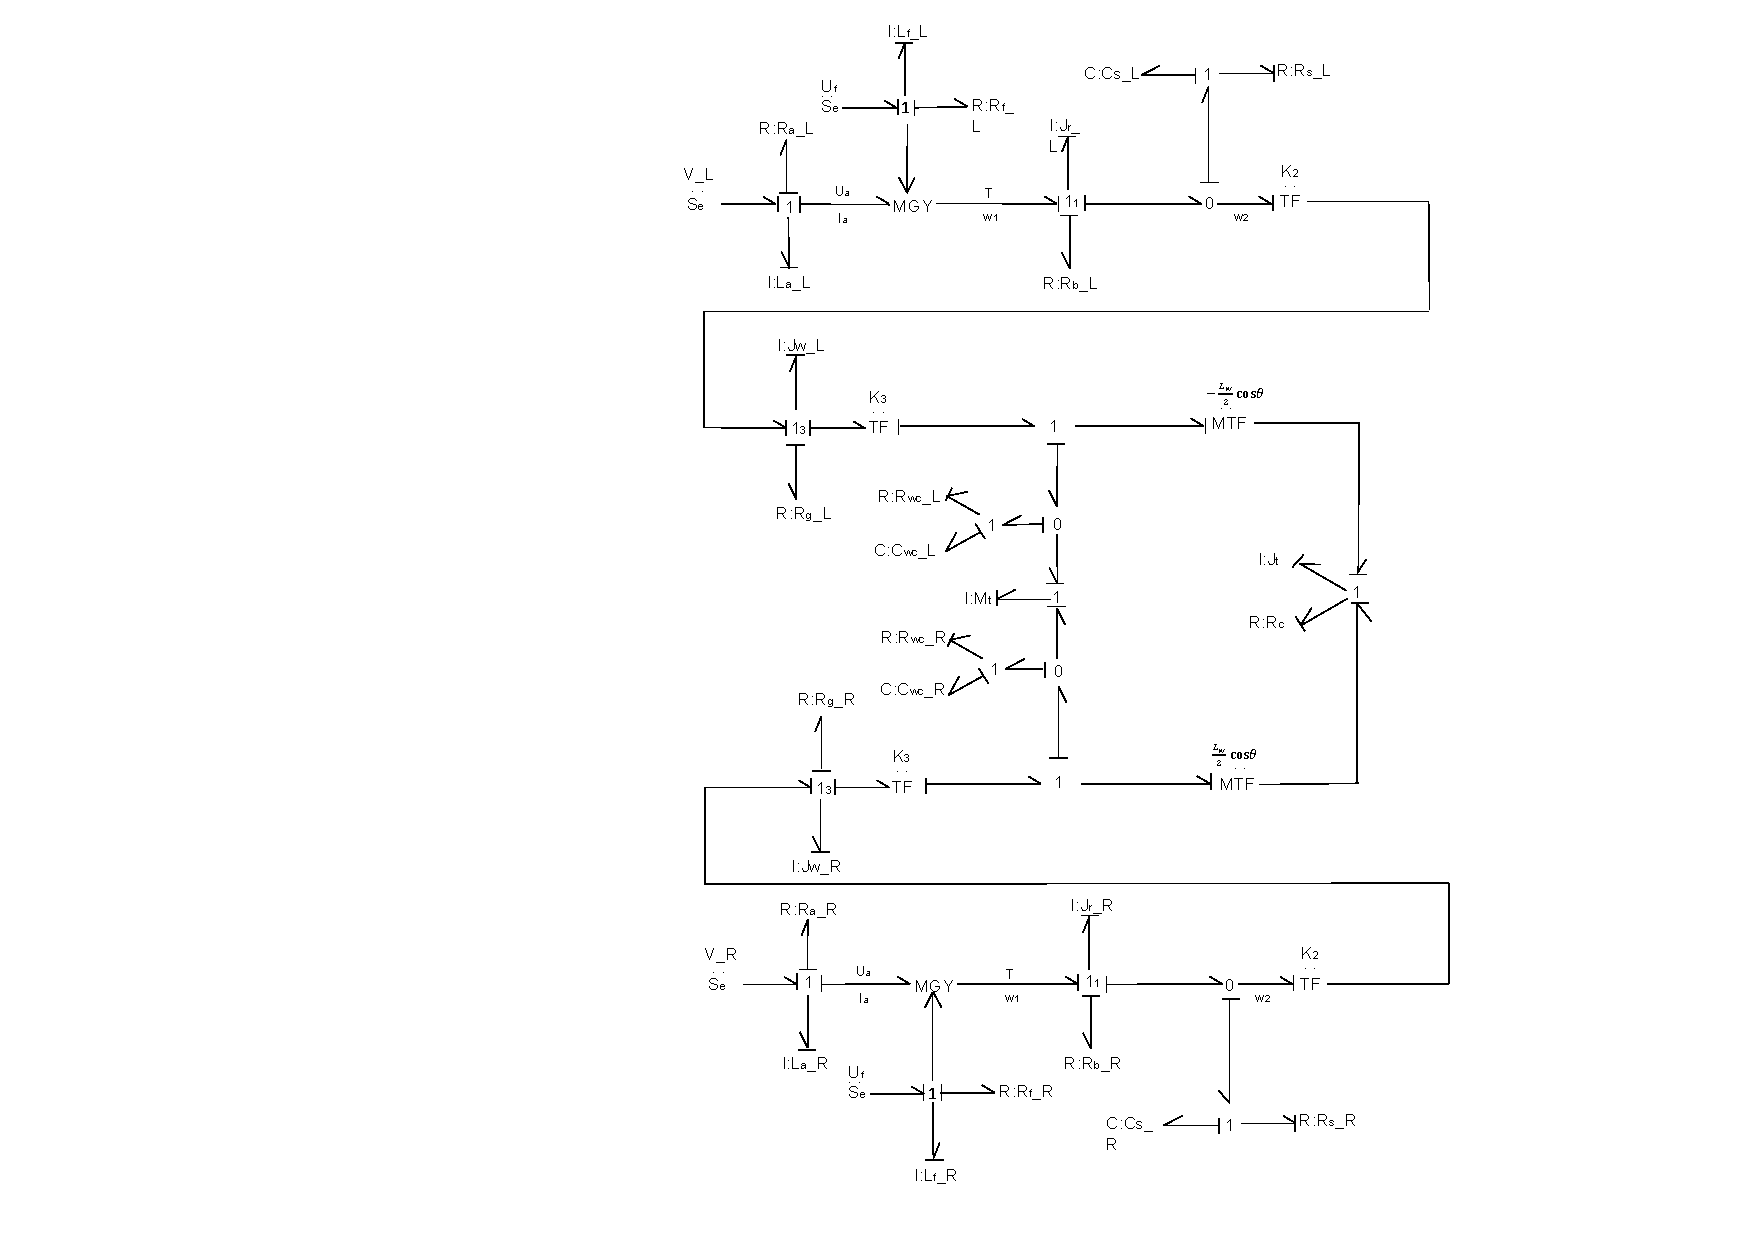
\includegraphics[width=1.2\textwidth,angle=90]{fig/part2_bond.pdf}
	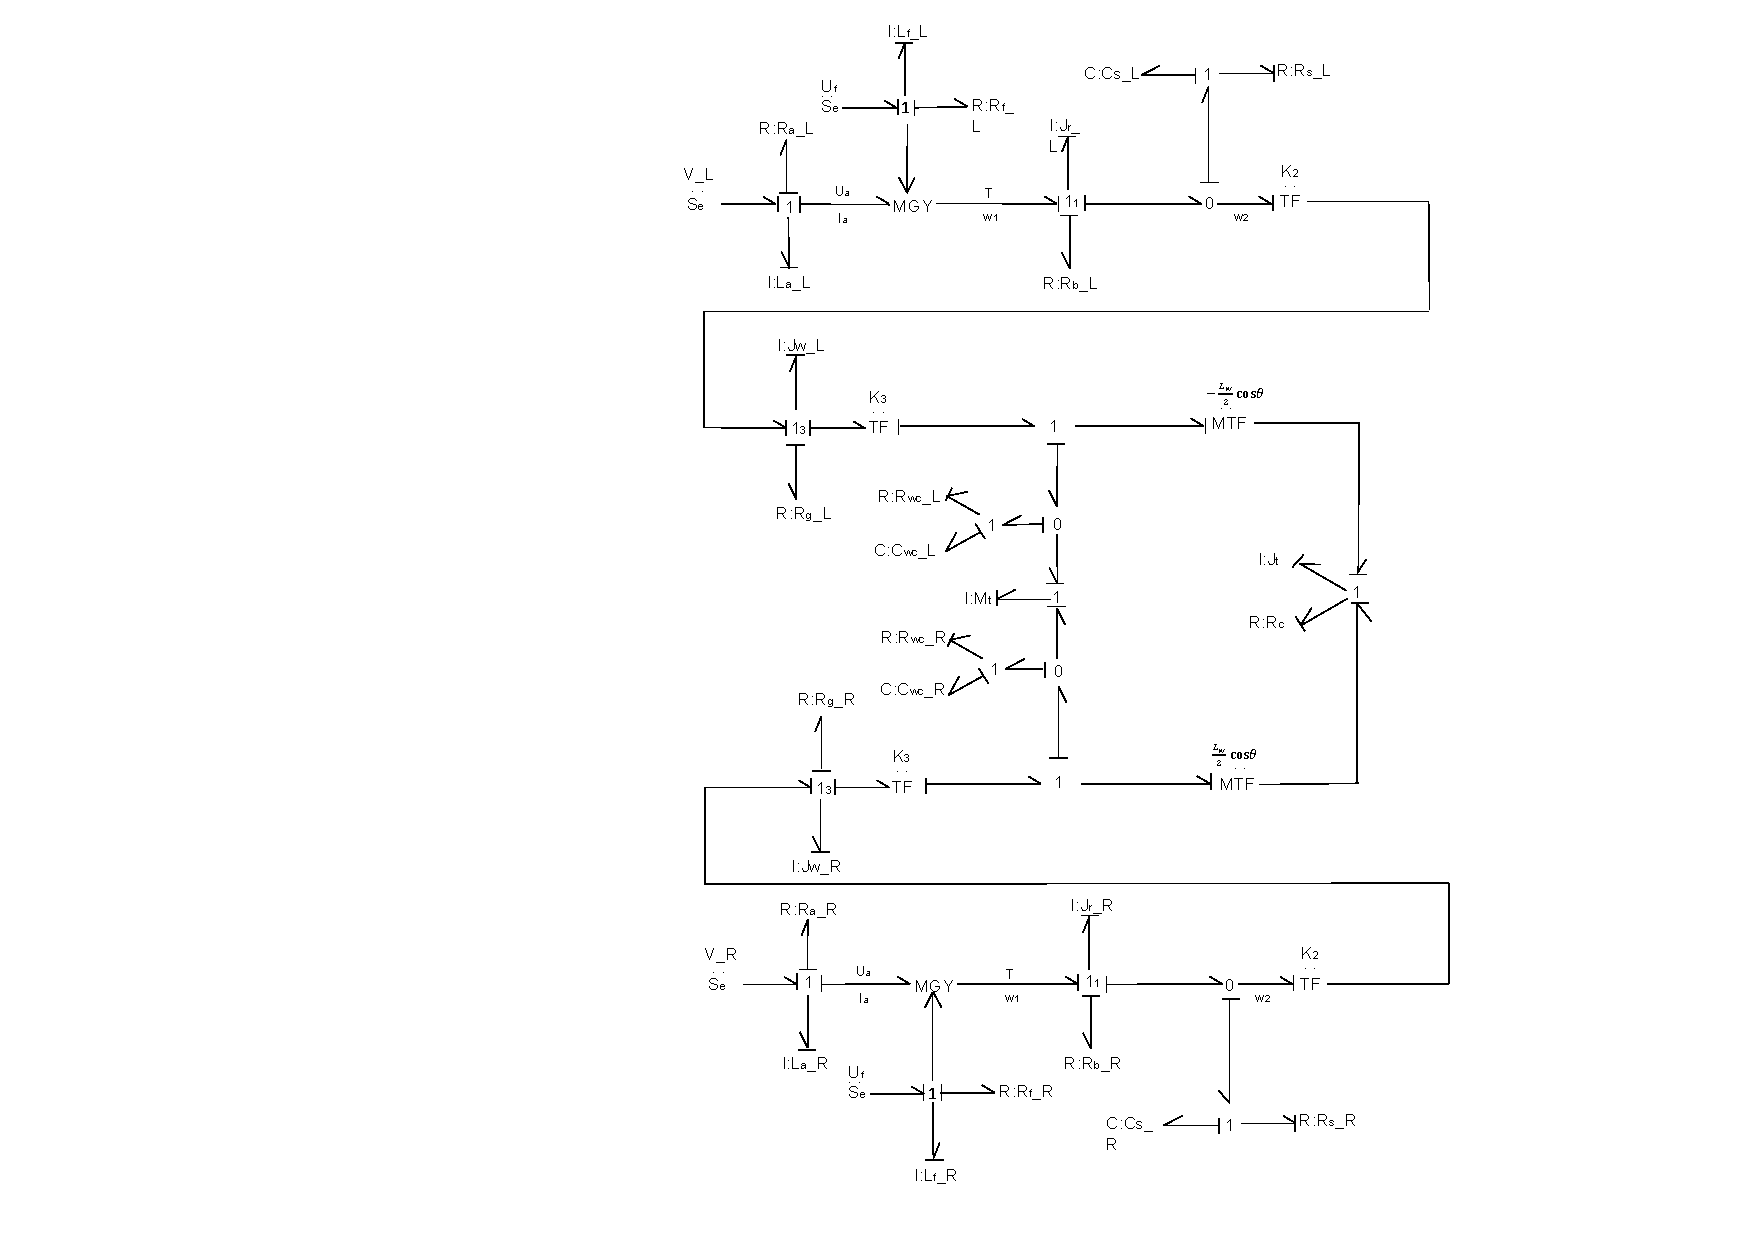
\includegraphics[width=1.05\textwidth]{fig/part2_bond.pdf}
	\caption{简化总体键合图。}\label{fig:part2_bond}
\end{figure*}
%%%%%%%%%%%%%%%%%

